\documentclass[tikz,border=8pt]{standalone}
\usepackage[utf8]{inputenc}\usetikzlibrary{positioning,fit,arrows.meta,shapes.geometric}
\definecolor{navy}{HTML}{17365D}\definecolor{teal}{HTML}{1F7A8C}\definecolor{soft}{HTML}{EAF4F6}
\tikzset{actor/.style={draw=navy,rounded corners,fill=white,minimum width=3.3cm,minimum height=.75cm,font=\bfseries\small},usecase/.style={draw=teal,ellipse,fill=soft,minimum width=6.2cm,minimum height=.75cm,align=center,font=\small},link/.style={draw=navy,-{Latex[length=2mm]},thin}}
\begin{document}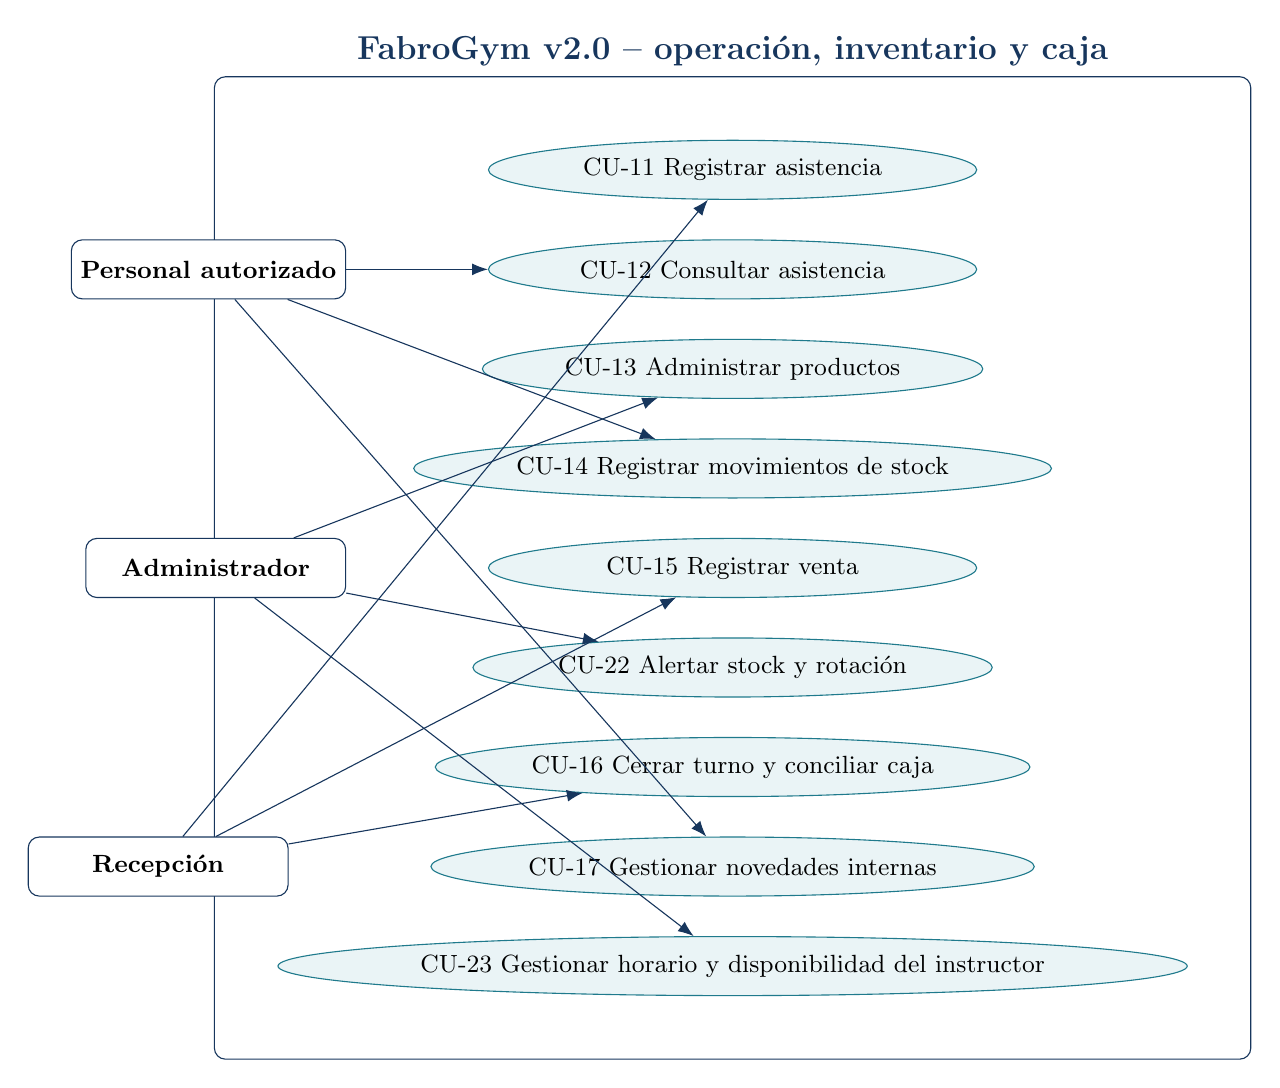
\begin{tikzpicture}[node distance=5mm and 16mm]
\node[usecase] (c11) {CU-11 Registrar asistencia};
\node[usecase,below=of c11] (c12) {CU-12 Consultar asistencia};
\node[usecase,below=of c12] (c13) {CU-13 Administrar productos};
\node[usecase,below=of c13] (c14) {CU-14 Registrar movimientos de stock};
\node[usecase,below=of c14] (c15) {CU-15 Registrar venta};
\node[usecase,below=of c15] (c22) {CU-22 Alertar stock y rotación};
\node[usecase,below=of c22] (c16) {CU-16 Cerrar turno y conciliar caja};
\node[usecase,below=of c16] (c17) {CU-17 Gestionar novedades internas};
\node[usecase,below=of c17] (c23) {CU-23 Gestionar horario y disponibilidad del instructor};
\node[draw=navy,rounded corners,fit=(c11)(c23),inner sep=8mm,label={[font=\bfseries\large,text=navy]above:FabroGym v2.0 -- operación, inventario y caja}] {};
\node[actor,left=18mm of c12] (pa) {Personal autorizado};
\node[actor,left=18mm of c15] (ad) {Administrador};
\node[actor,left=18mm of c17] (re) {Recepción};
\foreach \x in {c12,c14,c17}\draw[link] (pa)--(\x);
\foreach \x in {c13,c22,c23}\draw[link] (ad)--(\x);
\foreach \x in {c11,c15,c16}\draw[link] (re)--(\x);
\end{tikzpicture}\end{document}
